\documentclass{beamer}
\usepackage{gnuplot-lua-tikz}
\usepackage{caption}
\usetheme{Warsaw}
\DeclareGraphicsRule{.1}{mps}{*}{}

\title{Level 4 Project Presentation \\ A lightweight protocol for constrained devices for use in the Internet of
Things paradigm}
\author{Fergus Leahy}


\begin{document}
\maketitle


\begin{frame}
  \frametitle{Overview}
  \tableofcontents{}
\end{frame}


\section{What is the Internet of Things?} % (fold)
  \label{sec:introduction}
  \begin{frame}[t]\frametitle{What is the Internet of Things?}
  \only<1>{
    \begin{itemize}
      \item [--] \textbf{1999: RFID}
      \begin{itemize}
        \item Originally coined by Kevin Ashton, when managing company supply chain using RFID in 1999.
        \item Never really took off.
      \end{itemize}
    \end{itemize}
    }
  	\begin{itemize}
      \item<2->[--] \textbf{2013: Year of Internet of Things}
      \begin{itemize}
        \item Advent of cheap, low-power and small constrained devices.
        \item Consumer Electronics Show 2013
        \item Smart fridges, Smart watches, Smart washing machines, Smart scales, Smart cars, Smart Things and Smart ... plants?
        \item Plug something into the Internet, it's now smart.
        \item Creates an Internet of Things which can notify you when your wash cycle has complete, your milk has gone off and your plants about to bite the dust.
      \end{itemize}
    \end{itemize}
\only<2>{
    \begin{figure}[htb]
    \begin{minipage}{0.3\textwidth}
      \centering
        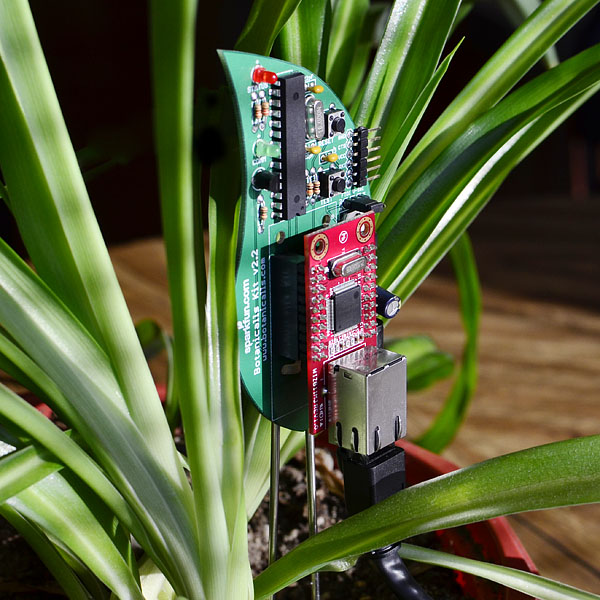
\includegraphics[scale=0.45]{presentation/img/smart-plant.jpg}
      \end{minipage}%
      \begin{minipage}{0.3\textwidth}
        \centering
          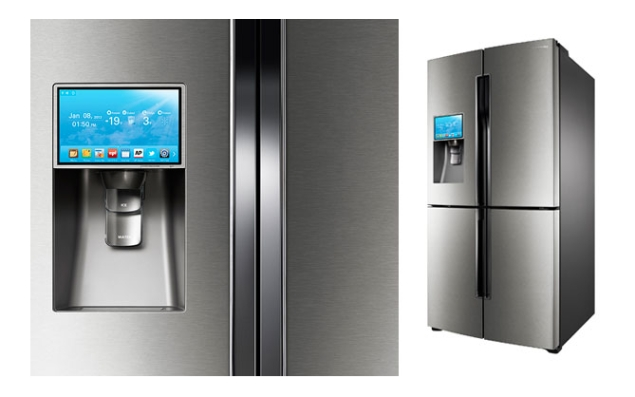
\includegraphics[scale=0.2]{presentation/img/smart-fridge.jpg}
      \end{minipage}%
      \begin{minipage}{0.3\textwidth}
        \centering
          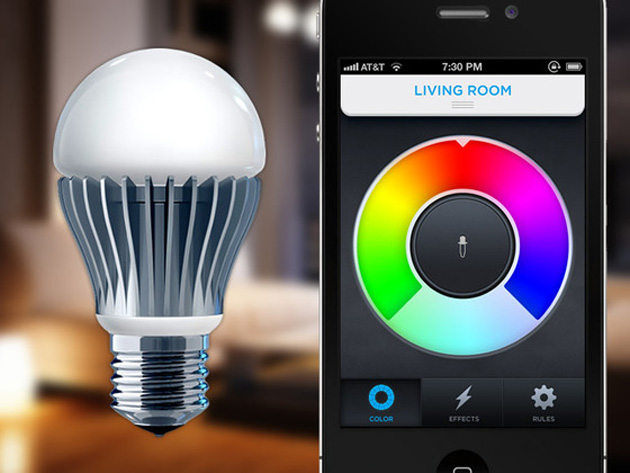
\includegraphics[scale=0.1]{presentation/img/smart-light.jpg}
      \end{minipage}
    \end{figure}
}  \end{frame}

  \begin{frame}[t]\frametitle{The bigger picture}
  \begin{itemize}
    \item Combine these cheap, small individual Things to create an autonomous network of devices.
    \item A network of devices which can sense, think and react to the environment.
    \item Relates to Wireless Sensor networks.
    \item More than just singular, simple actions, e.g.,
    \begin{itemize}
      \item Alarm set for 7.30AM, coffee machines turns on, blinds slowly open.
      \item House sensing user location, adjusting lighting and heating.
      \item Plants automatically watered based on soil moisture, weather patterns. 
    \end{itemize}
  \end{itemize}
  \end{frame}

\begin{frame}[t]\frametitle{Why?}
\begin{itemize}
  \item<1-> [--] \textbf{Not just a case of being lazy...}
  \item<2-> [--] \textbf{The Internet of People}
\begin{itemize}
  \item Internet in 2009 was 500 exabytes (that's 500 BILLION gigabytes), of which 70\% was contributed to by users
  \item Users are bad at data entry.
  \item Devices are reliable and accurate.
\end{itemize}
\item<3-> [--] \textbf{Smarter decisions}
  \begin{itemize}
      \item workload, complex decisions, saves resources, security
  \end{itemize}
\end{itemize}
\end{frame}


\section{What's wrong?} % (fold)
\begin{frame}[t]\frametitle{What's wrong, hasn't this been solved already?}
\label{sec:what_s_wrong_}
\begin{itemize}
  \item<1-> [--] \textbf{Eco-system is full of individual ``Things''}
  \begin{itemize}
    \item Hobbyist's ``Things'' vs Manufacturer's ``Things''.
    \item Simple, singular, heterogeneous network of devices.
    \item Constrained resources: battery, 8/16MHz CPU, ~40K ROM, ~10K RAM.
    \item Some open source efforts are trying...xAP, SmartThings.
    \item Existing protocols are too heavyweight/un-suited to constrained devices: JMS, TCP, HTTP,etc.
    \item IETF are pushing through new standards, CoRE \& CoAP, early days.
  \end{itemize}
  \item<2-> [--] \textbf{No simple, scalable solution for connecting these different types of ``Things'' together}
\end{itemize}
\end{frame}

\begin{frame}[t]\frametitle{Example attempts}

\begin{itemize}
    \item<1-> [--] \textbf{xAP: eXtensible Application Protocol}
  \begin{itemize}
    \item Heterogeneous network of devices can easily join, listen in and respond to what they're interested in.
    \item Distributed architecture, no central point of failure.
    \item Devices can easily join a network.
    \item Built on top of a multicast unreliable network.
    \item Devices broadcast ALL data, limited scalability.
  \end{itemize}
  \item<2-> [--] \textbf{SmartThings}
  \begin{itemize}
    \item Making existing objects smart by connecting them to a hub via low-power radio (Zigbee)
    \item Creating apps for your everyday things, user intervention.
    \item Cloud first, devices ``wired'' together in the cloud, hub just a gateway.
    \item Reliability \& Security...
    \item Yet to really open source the project
  \end{itemize}
\end{itemize}
\end{frame}
% section what_s_wrong_ (end)

\section{How can it be solved?} % (fold)
\label{sec:how_to_solve_it}
\begin{frame}[t]\frametitle{A new protocol}
\begin{itemize}
  \item [--] \textbf{Create a lightweight scalable protocol}
  \item [--] \textbf{Break the Internet of Things down to three basic roles}
  \begin{itemize}
    \item Sensor, the see-er
    \item Actuator, the do-er
    \item Controller, the brains
  \end{itemize}
  \item [--] \textbf{Distributed architecture with selective broadcasting}
  \begin{itemize}
    \item IoT is distributed in nature, no central point of failure.
    \item Broadcast needed for discovering devices.
  \end{itemize}
  \item [--] \textbf{Use an un-reliable connection and build reliability selectively on top}
  \begin{itemize}
    \item Full reliability is heavyweight e.g., TCP
    \item Ephemeral data
    \item Reliability of connection handling \& commands, timeouts \& PINGs for liveness
  \end{itemize}
\end{itemize}
\end{frame}

\begin{frame}[t]\frametitle{Implementation Target Platform}
\begin{itemize}
  \item [--] \textbf{A variety of different platforms to target}
  \begin{itemize}
    \item Arduino, TelosB, Raspberry Pi, Netduino, MSP430 Launchpad,
  \end{itemize}
  \only<2>{
  \item [--]\textbf{Original Platform: Arduino}
  \begin{itemize}
    \item 16MHz CPU, 2KB of RAM, 32KB ROM
    \item Huge following, open source, lots of copies, great online resources
    \item BUT no hardware interrupts from network interface...? Polling... 
  \end{itemize}}
  \only<3>{
  \item [--] \textbf{Final Platform: TelosB}
  \begin{itemize}
    \item Wireless Network Sensor platform, well tested device in academia
    \item 8MHz, 10KB RAM, 48KB ROM + low-power radio
    \item Several OSs to choose from: Contiki \& TinyOS + more...
    \item Contiki chosen, protothreads + events, uIP and Cooja
  \end{itemize}}
\end{itemize}
\only<3>{
\begin{figure}[htb]
      \centering
        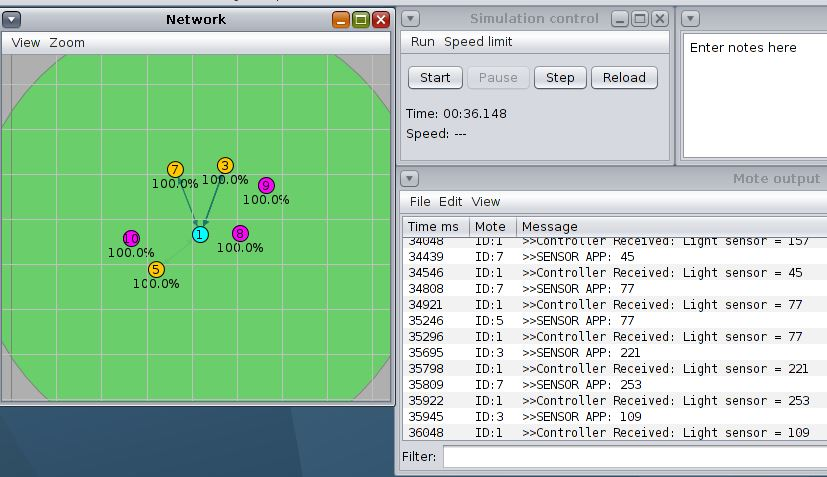
\includegraphics[scale=0.25]{evaluation/img/logTest.jpg}
    \end{figure}}
\end{frame}

\begin{frame}[t]\frametitle{Implementation overview}
% section how_to_solve_it (end)
\begin{itemize}
  \item [--] \textbf{IoT Protocol}
  \begin{itemize}
    \item Run over UDP
    \item 10 connections per device (due to RAM constraints)
    \item Event based API of applications on top
  \end{itemize}
  \end{itemize}

\begin{figure}[h!]
\centering
\includegraphics[scale=0.2]{implementation/img/system_architecture.1}
\caption{Overall system architecture}
\label{fig:system_architecture}
\end{figure}
     
\end{frame}


\section{Comparison} % (fold)
\label{sec:comparison}
\begin{frame}[t]\frametitle{How does this measure up?}
\begin{itemize}
  \item Consumes around 1Kbyte ROM and RAM with 10 connections
  \item Scales well as number of devices increases
\end{itemize}
\only<2>{
\begin{itemize}
  \item Comparison to xAP
  \begin{itemize}
    \item 2 scenarios
      \begin{itemize}
       \item 3 devices, 1 controller, 1 sensors, 1 actuators
       \item 5 devices, 1 controller, 2 sensors, 2 actuators
    \end{itemize} 
    \item Sensors sense every 1 second and ping every 10 seconds
    \item Controllers send commands to actuators every 15 seconds
    \item One minute period
  \end{itemize}
\end{itemize}
  }
\end{frame}

\begin{frame}
\begin{center}
\begin{figure}[h]
\tikzstyle{every node}=[font=\scriptsize]
\tikzset{every picture/.style={scale=0.67}}%
\begin{minipage}{.5\textwidth}
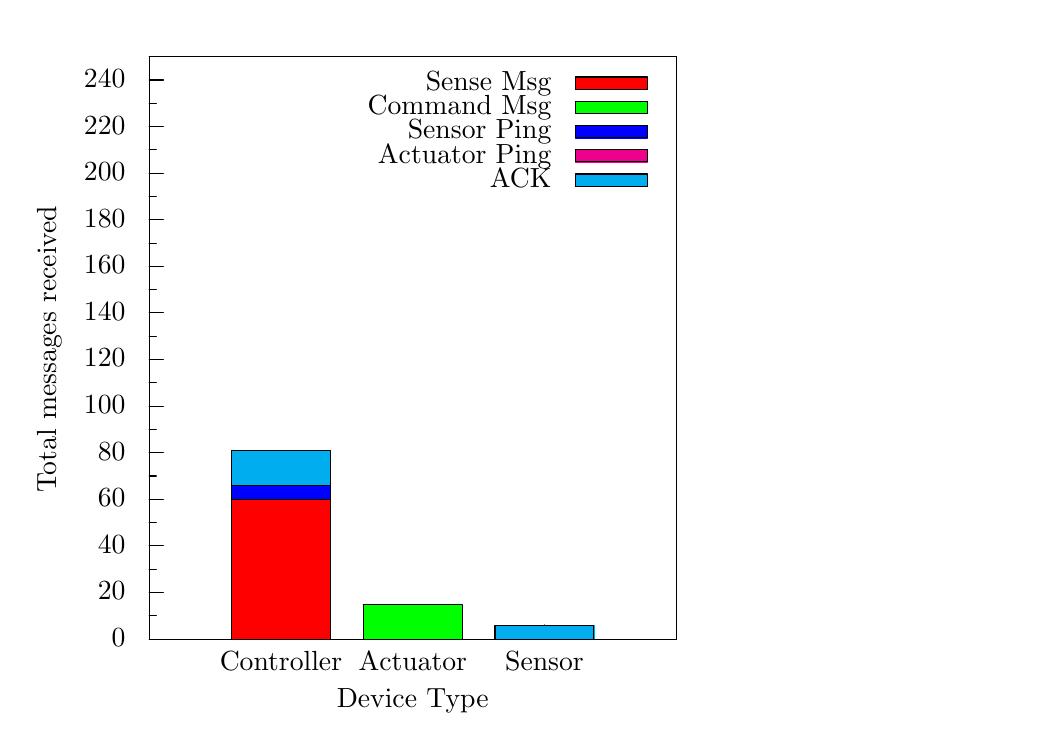
\begin{tikzpicture}[gnuplot]
%% generated with GNUPLOT 4.7p0 (Lua 5.1; terminal rev. 99, script rev. 100)
%% Wed 15 May 2013 18:37:35 BST
\gpsolidlines
\path (0.000,0.000) rectangle (12.500,8.750);
\gpcolor{color=gp lt color border}
\gpsetlinetype{gp lt border}
\gpsetlinewidth{1.00}
\draw[gp path] (1.504,0.985)--(1.684,0.985);
\node[gp node right] at (1.320,0.985) { 0};
\draw[gp path] (1.504,1.281)--(1.594,1.281);
\draw[gp path] (1.504,1.577)--(1.684,1.577);
\node[gp node right] at (1.320,1.577) { 20};
\draw[gp path] (1.504,1.873)--(1.594,1.873);
\draw[gp path] (1.504,2.168)--(1.684,2.168);
\node[gp node right] at (1.320,2.168) { 40};
\draw[gp path] (1.504,2.464)--(1.594,2.464);
\draw[gp path] (1.504,2.760)--(1.684,2.760);
\node[gp node right] at (1.320,2.760) { 60};
\draw[gp path] (1.504,3.056)--(1.594,3.056);
\draw[gp path] (1.504,3.352)--(1.684,3.352);
\node[gp node right] at (1.320,3.352) { 80};
\draw[gp path] (1.504,3.648)--(1.594,3.648);
\draw[gp path] (1.504,3.943)--(1.684,3.943);
\node[gp node right] at (1.320,3.943) { 100};
\draw[gp path] (1.504,4.239)--(1.594,4.239);
\draw[gp path] (1.504,4.535)--(1.684,4.535);
\node[gp node right] at (1.320,4.535) { 120};
\draw[gp path] (1.504,4.831)--(1.594,4.831);
\draw[gp path] (1.504,5.127)--(1.684,5.127);
\node[gp node right] at (1.320,5.127) { 140};
\draw[gp path] (1.504,5.423)--(1.594,5.423);
\draw[gp path] (1.504,5.718)--(1.684,5.718);
\node[gp node right] at (1.320,5.718) { 160};
\draw[gp path] (1.504,6.014)--(1.594,6.014);
\draw[gp path] (1.504,6.310)--(1.684,6.310);
\node[gp node right] at (1.320,6.310) { 180};
\draw[gp path] (1.504,6.606)--(1.594,6.606);
\draw[gp path] (1.504,6.902)--(1.684,6.902);
\node[gp node right] at (1.320,6.902) { 200};
\draw[gp path] (1.504,7.198)--(1.594,7.198);
\draw[gp path] (1.504,7.493)--(1.684,7.493);
\node[gp node right] at (1.320,7.493) { 220};
\draw[gp path] (1.504,7.789)--(1.594,7.789);
\draw[gp path] (1.504,8.085)--(1.684,8.085);
\node[gp node right] at (1.320,8.085) { 240};
\draw[gp path] (1.504,8.381)--(1.594,8.381);
\draw[gp path] (3.177,0.985)--(3.177,1.165);
\node[gp node center] at (3.177,0.677) {Controller};
\draw[gp path] (4.851,0.985)--(4.851,1.165);
\node[gp node center] at (4.851,0.677) {Actuator};
\draw[gp path] (6.524,0.985)--(6.524,1.165);
\node[gp node center] at (6.524,0.677) {Sensor};
\draw[gp path] (1.504,8.381)--(1.504,0.985)--(8.197,0.985)--(8.197,8.381)--cycle;
\node[gp node center,rotate=-270] at (0.246,4.683) {Total messages received};
\node[gp node center] at (4.850,0.215) {Device Type};
\node[gp node right] at (6.729,8.047) {Sense Msg};
\gpfill{color=gp lt color 0} (6.913,7.970)--(7.829,7.970)--(7.829,8.124)--(6.913,8.124)--cycle;
\gpsetlinetype{gp lt plot 0}
\draw[gp path] (6.913,7.970)--(7.829,7.970)--(7.829,8.124)--(6.913,8.124)--cycle;
\gpfill{color=gp lt color 0} (2.550,0.985)--(3.806,0.985)--(3.806,2.761)--(2.550,2.761)--cycle;
\draw[gp path] (2.550,0.985)--(2.550,2.760)--(3.805,2.760)--(3.805,0.985)--cycle;
\node[gp node right] at (6.729,7.739) {Command Msg};
\gpfill{color=gp lt color 1} (6.913,7.662)--(7.829,7.662)--(7.829,7.816)--(6.913,7.816)--cycle;
\gpsetlinetype{gp lt plot 1}
\draw[gp path] (6.913,7.662)--(7.829,7.662)--(7.829,7.816)--(6.913,7.816)--cycle;
\gpfill{color=gp lt color 1} (2.550,2.760)--(3.806,2.760)--(3.806,2.761)--(2.550,2.761)--cycle;
\draw[gp path] (2.550,2.760)--(3.805,2.760)--cycle;
\gpfill{color=gp lt color 1} (4.223,0.985)--(5.479,0.985)--(5.479,1.430)--(4.223,1.430)--cycle;
\draw[gp path] (4.223,0.985)--(4.223,1.429)--(5.478,1.429)--(5.478,0.985)--cycle;
\node[gp node right] at (6.729,7.431) {Sensor Ping};
\gpfill{color=gp lt color 2} (6.913,7.354)--(7.829,7.354)--(7.829,7.508)--(6.913,7.508)--cycle;
\gpsetlinetype{gp lt plot 2}
\draw[gp path] (6.913,7.354)--(7.829,7.354)--(7.829,7.508)--(6.913,7.508)--cycle;
\gpfill{color=gp lt color 2} (2.550,2.760)--(3.806,2.760)--(3.806,2.939)--(2.550,2.939)--cycle;
\draw[gp path] (2.550,2.760)--(2.550,2.938)--(3.805,2.938)--(3.805,2.760)--cycle;
\gpfill{color=gp lt color 2} (4.223,1.429)--(5.479,1.429)--(5.479,1.430)--(4.223,1.430)--cycle;
\draw[gp path] (4.223,1.429)--(5.478,1.429)--cycle;
\node[gp node right] at (6.729,7.123) {Actuator Ping};
\gpfill{color=gp lt color 3} (6.913,7.046)--(7.829,7.046)--(7.829,7.200)--(6.913,7.200)--cycle;
\gpsetlinetype{gp lt plot 3}
\draw[gp path] (6.913,7.046)--(7.829,7.046)--(7.829,7.200)--(6.913,7.200)--cycle;
\gpfill{color=gp lt color 3} (2.550,2.938)--(3.806,2.938)--(3.806,2.939)--(2.550,2.939)--cycle;
\draw[gp path] (2.550,2.938)--(3.805,2.938)--cycle;
\gpfill{color=gp lt color 3} (4.223,1.429)--(5.479,1.429)--(5.479,1.430)--(4.223,1.430)--cycle;
\draw[gp path] (4.223,1.429)--(5.478,1.429)--cycle;
\node[gp node right] at (6.729,6.815) {ACK};
\gpfill{color=gp lt color 4} (6.913,6.738)--(7.829,6.738)--(7.829,6.892)--(6.913,6.892)--cycle;
\gpsetlinetype{gp lt plot 4}
\draw[gp path] (6.913,6.738)--(7.829,6.738)--(7.829,6.892)--(6.913,6.892)--cycle;
\gpfill{color=gp lt color 4} (2.550,2.938)--(3.806,2.938)--(3.806,3.382)--(2.550,3.382)--cycle;
\draw[gp path] (2.550,2.938)--(2.550,3.381)--(3.805,3.381)--(3.805,2.938)--cycle;
\gpfill{color=gp lt color 4} (4.223,1.429)--(5.479,1.429)--(5.479,1.430)--(4.223,1.430)--cycle;
\draw[gp path] (4.223,1.429)--(5.478,1.429)--cycle;
\gpfill{color=gp lt color 4} (5.896,0.985)--(7.152,0.985)--(7.152,1.164)--(5.896,1.164)--cycle;
\draw[gp path] (5.896,0.985)--(5.896,1.163)--(7.151,1.163)--(7.151,0.985)--cycle;
\gpsetlinetype{gp lt border}
\draw[gp path] (1.504,8.381)--(1.504,0.985)--(8.197,0.985)--(8.197,8.381)--cycle;
%% coordinates of the plot area
\gpdefrectangularnode{gp plot 1}{\pgfpoint{1.504cm}{0.985cm}}{\pgfpoint{8.197cm}{8.381cm}}
\end{tikzpicture}
%% gnuplot variables

\caption{IoT}
\label{graph:IoT2}
\end{minipage}%
\begin{minipage}{.5\textwidth}
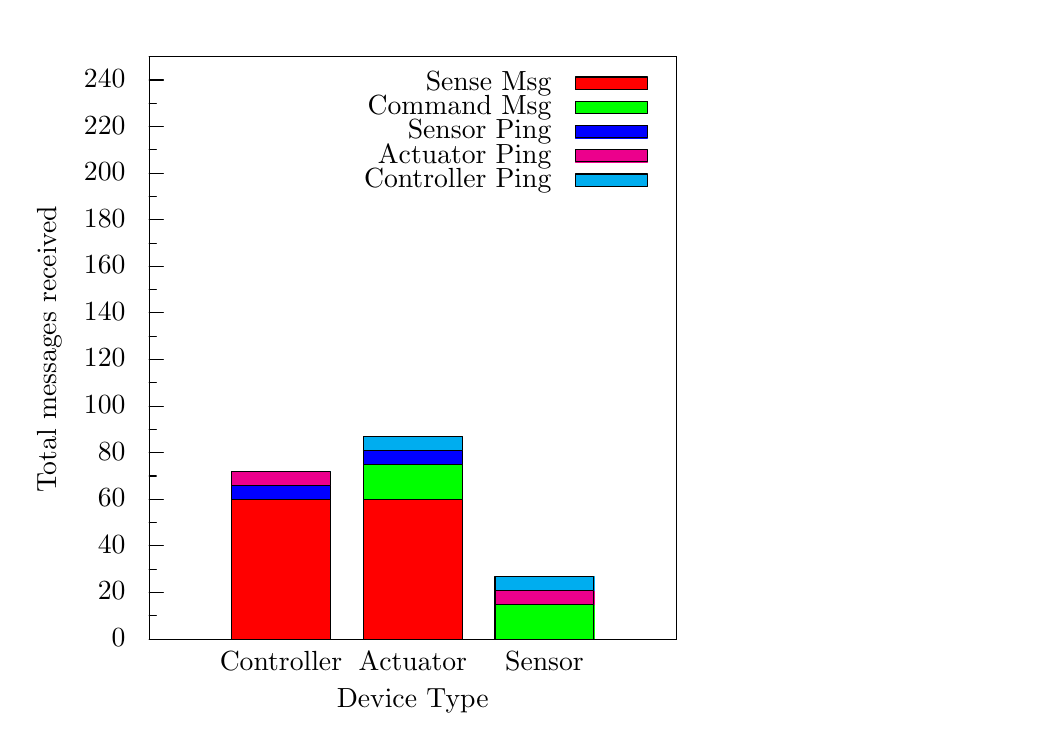
\begin{tikzpicture}[gnuplot]
%% generated with GNUPLOT 4.7p0 (Lua 5.1; terminal rev. 99, script rev. 100)
%% Fri 26 Apr 2013 15:19:36 BST
\gpsolidlines
\path (0.000,0.000) rectangle (12.500,8.750);
\gpcolor{color=gp lt color border}
\gpsetlinetype{gp lt border}
\gpsetlinewidth{1.00}
\draw[gp path] (1.504,0.985)--(1.684,0.985);
\node[gp node right] at (1.320,0.985) { 0};
\draw[gp path] (1.504,1.281)--(1.594,1.281);
\draw[gp path] (1.504,1.577)--(1.684,1.577);
\node[gp node right] at (1.320,1.577) { 20};
\draw[gp path] (1.504,1.873)--(1.594,1.873);
\draw[gp path] (1.504,2.168)--(1.684,2.168);
\node[gp node right] at (1.320,2.168) { 40};
\draw[gp path] (1.504,2.464)--(1.594,2.464);
\draw[gp path] (1.504,2.760)--(1.684,2.760);
\node[gp node right] at (1.320,2.760) { 60};
\draw[gp path] (1.504,3.056)--(1.594,3.056);
\draw[gp path] (1.504,3.352)--(1.684,3.352);
\node[gp node right] at (1.320,3.352) { 80};
\draw[gp path] (1.504,3.648)--(1.594,3.648);
\draw[gp path] (1.504,3.943)--(1.684,3.943);
\node[gp node right] at (1.320,3.943) { 100};
\draw[gp path] (1.504,4.239)--(1.594,4.239);
\draw[gp path] (1.504,4.535)--(1.684,4.535);
\node[gp node right] at (1.320,4.535) { 120};
\draw[gp path] (1.504,4.831)--(1.594,4.831);
\draw[gp path] (1.504,5.127)--(1.684,5.127);
\node[gp node right] at (1.320,5.127) { 140};
\draw[gp path] (1.504,5.423)--(1.594,5.423);
\draw[gp path] (1.504,5.718)--(1.684,5.718);
\node[gp node right] at (1.320,5.718) { 160};
\draw[gp path] (1.504,6.014)--(1.594,6.014);
\draw[gp path] (1.504,6.310)--(1.684,6.310);
\node[gp node right] at (1.320,6.310) { 180};
\draw[gp path] (1.504,6.606)--(1.594,6.606);
\draw[gp path] (1.504,6.902)--(1.684,6.902);
\node[gp node right] at (1.320,6.902) { 200};
\draw[gp path] (1.504,7.198)--(1.594,7.198);
\draw[gp path] (1.504,7.493)--(1.684,7.493);
\node[gp node right] at (1.320,7.493) { 220};
\draw[gp path] (1.504,7.789)--(1.594,7.789);
\draw[gp path] (1.504,8.085)--(1.684,8.085);
\node[gp node right] at (1.320,8.085) { 240};
\draw[gp path] (1.504,8.381)--(1.594,8.381);
\draw[gp path] (3.177,0.985)--(3.177,1.165);
\node[gp node center] at (3.177,0.677) {Controller};
\draw[gp path] (4.851,0.985)--(4.851,1.165);
\node[gp node center] at (4.851,0.677) {Actuator};
\draw[gp path] (6.524,0.985)--(6.524,1.165);
\node[gp node center] at (6.524,0.677) {Sensor};
\draw[gp path] (1.504,8.381)--(1.504,0.985)--(8.197,0.985)--(8.197,8.381)--cycle;
\node[gp node center,rotate=-270] at (0.246,4.683) {Total messages received};
\node[gp node center] at (4.850,0.215) {Device Type};
\node[gp node right] at (6.729,8.047) {Sense Msg};
\gpfill{color=gp lt color 0} (6.913,7.970)--(7.829,7.970)--(7.829,8.124)--(6.913,8.124)--cycle;
\gpsetlinetype{gp lt plot 0}
\draw[gp path] (6.913,7.970)--(7.829,7.970)--(7.829,8.124)--(6.913,8.124)--cycle;
\gpfill{color=gp lt color 0} (2.550,0.985)--(3.806,0.985)--(3.806,2.761)--(2.550,2.761)--cycle;
\draw[gp path] (2.550,0.985)--(2.550,2.760)--(3.805,2.760)--(3.805,0.985)--cycle;
\gpfill{color=gp lt color 0} (4.223,0.985)--(5.479,0.985)--(5.479,2.761)--(4.223,2.761)--cycle;
\draw[gp path] (4.223,0.985)--(4.223,2.760)--(5.478,2.760)--(5.478,0.985)--cycle;
\node[gp node right] at (6.729,7.739) {Command Msg};
\gpfill{color=gp lt color 1} (6.913,7.662)--(7.829,7.662)--(7.829,7.816)--(6.913,7.816)--cycle;
\gpsetlinetype{gp lt plot 1}
\draw[gp path] (6.913,7.662)--(7.829,7.662)--(7.829,7.816)--(6.913,7.816)--cycle;
\gpfill{color=gp lt color 1} (2.550,2.760)--(3.806,2.760)--(3.806,2.761)--(2.550,2.761)--cycle;
\draw[gp path] (2.550,2.760)--(3.805,2.760)--cycle;
\gpfill{color=gp lt color 1} (4.223,2.760)--(5.479,2.760)--(5.479,3.205)--(4.223,3.205)--cycle;
\draw[gp path] (4.223,2.760)--(4.223,3.204)--(5.478,3.204)--(5.478,2.760)--cycle;
\gpfill{color=gp lt color 1} (5.896,0.985)--(7.152,0.985)--(7.152,1.430)--(5.896,1.430)--cycle;
\draw[gp path] (5.896,0.985)--(5.896,1.429)--(7.151,1.429)--(7.151,0.985)--cycle;
\node[gp node right] at (6.729,7.431) {Sensor Ping};
\gpfill{color=gp lt color 2} (6.913,7.354)--(7.829,7.354)--(7.829,7.508)--(6.913,7.508)--cycle;
\gpsetlinetype{gp lt plot 2}
\draw[gp path] (6.913,7.354)--(7.829,7.354)--(7.829,7.508)--(6.913,7.508)--cycle;
\gpfill{color=gp lt color 2} (2.550,2.760)--(3.806,2.760)--(3.806,2.939)--(2.550,2.939)--cycle;
\draw[gp path] (2.550,2.760)--(2.550,2.938)--(3.805,2.938)--(3.805,2.760)--cycle;
\gpfill{color=gp lt color 2} (4.223,3.204)--(5.479,3.204)--(5.479,3.382)--(4.223,3.382)--cycle;
\draw[gp path] (4.223,3.204)--(4.223,3.381)--(5.478,3.381)--(5.478,3.204)--cycle;
\gpfill{color=gp lt color 2} (5.896,1.429)--(7.152,1.429)--(7.152,1.430)--(5.896,1.430)--cycle;
\draw[gp path] (5.896,1.429)--(7.151,1.429)--cycle;
\node[gp node right] at (6.729,7.123) {Actuator Ping};
\gpfill{color=gp lt color 3} (6.913,7.046)--(7.829,7.046)--(7.829,7.200)--(6.913,7.200)--cycle;
\gpsetlinetype{gp lt plot 3}
\draw[gp path] (6.913,7.046)--(7.829,7.046)--(7.829,7.200)--(6.913,7.200)--cycle;
\gpfill{color=gp lt color 3} (2.550,2.938)--(3.806,2.938)--(3.806,3.116)--(2.550,3.116)--cycle;
\draw[gp path] (2.550,2.938)--(2.550,3.115)--(3.805,3.115)--(3.805,2.938)--cycle;
\gpfill{color=gp lt color 3} (4.223,3.381)--(5.479,3.381)--(5.479,3.382)--(4.223,3.382)--cycle;
\draw[gp path] (4.223,3.381)--(5.478,3.381)--cycle;
\gpfill{color=gp lt color 3} (5.896,1.429)--(7.152,1.429)--(7.152,1.607)--(5.896,1.607)--cycle;
\draw[gp path] (5.896,1.429)--(5.896,1.606)--(7.151,1.606)--(7.151,1.429)--cycle;
\node[gp node right] at (6.729,6.815) {Controller Ping};
\gpfill{color=gp lt color 4} (6.913,6.738)--(7.829,6.738)--(7.829,6.892)--(6.913,6.892)--cycle;
\gpsetlinetype{gp lt plot 4}
\draw[gp path] (6.913,6.738)--(7.829,6.738)--(7.829,6.892)--(6.913,6.892)--cycle;
\gpfill{color=gp lt color 4} (2.550,3.115)--(3.806,3.115)--(3.806,3.116)--(2.550,3.116)--cycle;
\draw[gp path] (2.550,3.115)--(3.805,3.115)--cycle;
\gpfill{color=gp lt color 4} (4.223,3.381)--(5.479,3.381)--(5.479,3.560)--(4.223,3.560)--cycle;
\draw[gp path] (4.223,3.381)--(4.223,3.559)--(5.478,3.559)--(5.478,3.381)--cycle;
\gpfill{color=gp lt color 4} (5.896,1.606)--(7.152,1.606)--(7.152,1.785)--(5.896,1.785)--cycle;
\draw[gp path] (5.896,1.606)--(5.896,1.784)--(7.151,1.784)--(7.151,1.606)--cycle;
\gpsetlinetype{gp lt border}
\draw[gp path] (1.504,8.381)--(1.504,0.985)--(8.197,0.985)--(8.197,8.381)--cycle;
%% coordinates of the plot area
\gpdefrectangularnode{gp plot 1}{\pgfpoint{1.504cm}{0.985cm}}{\pgfpoint{8.197cm}{8.381cm}}
\end{tikzpicture}
%% gnuplot variables

\caption{xAP}
\label{graph:IoT2}
\end{minipage}
\end{figure}
\end{center}
\end{frame}


\begin{frame}
\begin{figure}[h]
\centering
\tikzstyle{every node}=[font=\scriptsize]
\tikzset{every picture/.style={scale=0.67}}%
\begin{minipage}{.5\textwidth}
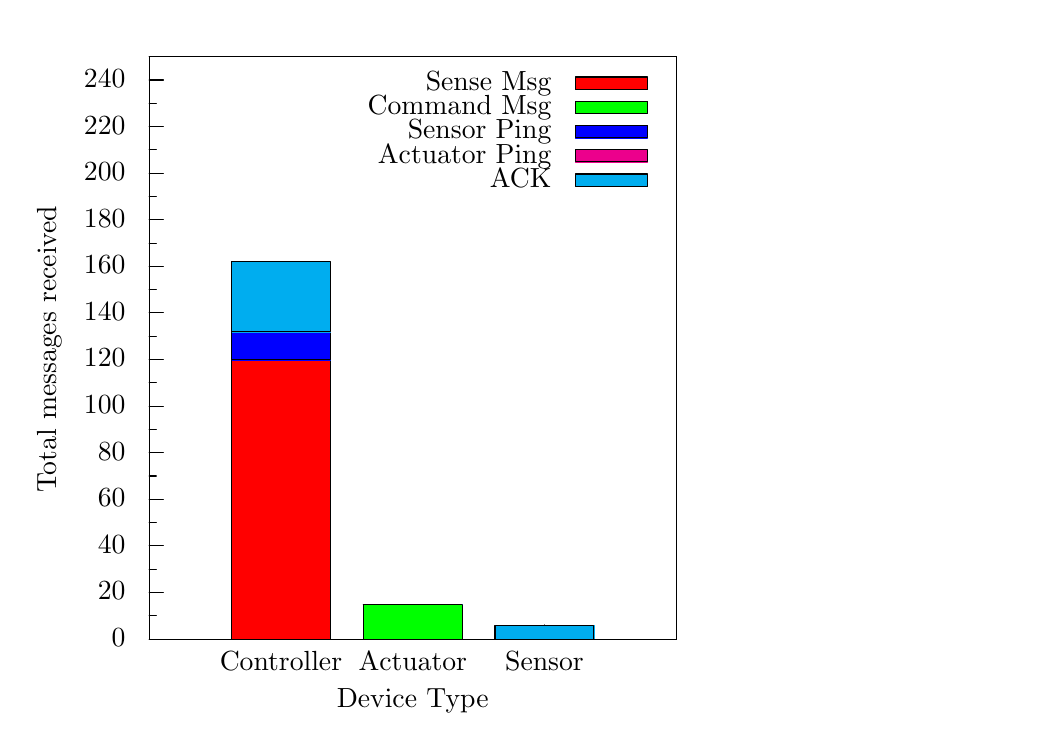
\begin{tikzpicture}[gnuplot]
%% generated with GNUPLOT 4.7p0 (Lua 5.1; terminal rev. 99, script rev. 100)
%% Fri 26 Apr 2013 15:19:36 BST
\gpsolidlines
\path (0.000,0.000) rectangle (12.500,8.750);
\gpcolor{color=gp lt color border}
\gpsetlinetype{gp lt border}
\gpsetlinewidth{1.00}
\draw[gp path] (1.504,0.985)--(1.684,0.985);
\node[gp node right] at (1.320,0.985) { 0};
\draw[gp path] (1.504,1.281)--(1.594,1.281);
\draw[gp path] (1.504,1.577)--(1.684,1.577);
\node[gp node right] at (1.320,1.577) { 20};
\draw[gp path] (1.504,1.873)--(1.594,1.873);
\draw[gp path] (1.504,2.168)--(1.684,2.168);
\node[gp node right] at (1.320,2.168) { 40};
\draw[gp path] (1.504,2.464)--(1.594,2.464);
\draw[gp path] (1.504,2.760)--(1.684,2.760);
\node[gp node right] at (1.320,2.760) { 60};
\draw[gp path] (1.504,3.056)--(1.594,3.056);
\draw[gp path] (1.504,3.352)--(1.684,3.352);
\node[gp node right] at (1.320,3.352) { 80};
\draw[gp path] (1.504,3.648)--(1.594,3.648);
\draw[gp path] (1.504,3.943)--(1.684,3.943);
\node[gp node right] at (1.320,3.943) { 100};
\draw[gp path] (1.504,4.239)--(1.594,4.239);
\draw[gp path] (1.504,4.535)--(1.684,4.535);
\node[gp node right] at (1.320,4.535) { 120};
\draw[gp path] (1.504,4.831)--(1.594,4.831);
\draw[gp path] (1.504,5.127)--(1.684,5.127);
\node[gp node right] at (1.320,5.127) { 140};
\draw[gp path] (1.504,5.423)--(1.594,5.423);
\draw[gp path] (1.504,5.718)--(1.684,5.718);
\node[gp node right] at (1.320,5.718) { 160};
\draw[gp path] (1.504,6.014)--(1.594,6.014);
\draw[gp path] (1.504,6.310)--(1.684,6.310);
\node[gp node right] at (1.320,6.310) { 180};
\draw[gp path] (1.504,6.606)--(1.594,6.606);
\draw[gp path] (1.504,6.902)--(1.684,6.902);
\node[gp node right] at (1.320,6.902) { 200};
\draw[gp path] (1.504,7.198)--(1.594,7.198);
\draw[gp path] (1.504,7.493)--(1.684,7.493);
\node[gp node right] at (1.320,7.493) { 220};
\draw[gp path] (1.504,7.789)--(1.594,7.789);
\draw[gp path] (1.504,8.085)--(1.684,8.085);
\node[gp node right] at (1.320,8.085) { 240};
\draw[gp path] (1.504,8.381)--(1.594,8.381);
\draw[gp path] (3.177,0.985)--(3.177,1.165);
\node[gp node center] at (3.177,0.677) {Controller};
\draw[gp path] (4.851,0.985)--(4.851,1.165);
\node[gp node center] at (4.851,0.677) {Actuator};
\draw[gp path] (6.524,0.985)--(6.524,1.165);
\node[gp node center] at (6.524,0.677) {Sensor};
\draw[gp path] (1.504,8.381)--(1.504,0.985)--(8.197,0.985)--(8.197,8.381)--cycle;
\node[gp node center,rotate=-270] at (0.246,4.683) {Total messages received};
\node[gp node center] at (4.850,0.215) {Device Type};
\node[gp node right] at (6.729,8.047) {Sense Msg};
\gpfill{color=gp lt color 0} (6.913,7.970)--(7.829,7.970)--(7.829,8.124)--(6.913,8.124)--cycle;
\gpsetlinetype{gp lt plot 0}
\draw[gp path] (6.913,7.970)--(7.829,7.970)--(7.829,8.124)--(6.913,8.124)--cycle;
\gpfill{color=gp lt color 0} (2.550,0.985)--(3.806,0.985)--(3.806,4.536)--(2.550,4.536)--cycle;
\draw[gp path] (2.550,0.985)--(2.550,4.535)--(3.805,4.535)--(3.805,0.985)--cycle;
\node[gp node right] at (6.729,7.739) {Command Msg};
\gpfill{color=gp lt color 1} (6.913,7.662)--(7.829,7.662)--(7.829,7.816)--(6.913,7.816)--cycle;
\gpsetlinetype{gp lt plot 1}
\draw[gp path] (6.913,7.662)--(7.829,7.662)--(7.829,7.816)--(6.913,7.816)--cycle;
\gpfill{color=gp lt color 1} (2.550,4.535)--(3.806,4.535)--(3.806,4.536)--(2.550,4.536)--cycle;
\draw[gp path] (2.550,4.535)--(3.805,4.535)--cycle;
\gpfill{color=gp lt color 1} (4.223,0.985)--(5.479,0.985)--(5.479,1.430)--(4.223,1.430)--cycle;
\draw[gp path] (4.223,0.985)--(4.223,1.429)--(5.478,1.429)--(5.478,0.985)--cycle;
\node[gp node right] at (6.729,7.431) {Sensor Ping};
\gpfill{color=gp lt color 2} (6.913,7.354)--(7.829,7.354)--(7.829,7.508)--(6.913,7.508)--cycle;
\gpsetlinetype{gp lt plot 2}
\draw[gp path] (6.913,7.354)--(7.829,7.354)--(7.829,7.508)--(6.913,7.508)--cycle;
\gpfill{color=gp lt color 2} (2.550,4.535)--(3.806,4.535)--(3.806,4.891)--(2.550,4.891)--cycle;
\draw[gp path] (2.550,4.535)--(2.550,4.890)--(3.805,4.890)--(3.805,4.535)--cycle;
\gpfill{color=gp lt color 2} (4.223,1.429)--(5.479,1.429)--(5.479,1.430)--(4.223,1.430)--cycle;
\draw[gp path] (4.223,1.429)--(5.478,1.429)--cycle;
\node[gp node right] at (6.729,7.123) {Actuator Ping};
\gpfill{color=gp lt color 3} (6.913,7.046)--(7.829,7.046)--(7.829,7.200)--(6.913,7.200)--cycle;
\gpsetlinetype{gp lt plot 3}
\draw[gp path] (6.913,7.046)--(7.829,7.046)--(7.829,7.200)--(6.913,7.200)--cycle;
\gpfill{color=gp lt color 3} (2.550,4.890)--(3.806,4.890)--(3.806,4.891)--(2.550,4.891)--cycle;
\draw[gp path] (2.550,4.890)--(3.805,4.890)--cycle;
\gpfill{color=gp lt color 3} (4.223,1.429)--(5.479,1.429)--(5.479,1.430)--(4.223,1.430)--cycle;
\draw[gp path] (4.223,1.429)--(5.478,1.429)--cycle;
\node[gp node right] at (6.729,6.815) {ACK};
\gpfill{color=gp lt color 4} (6.913,6.738)--(7.829,6.738)--(7.829,6.892)--(6.913,6.892)--cycle;
\gpsetlinetype{gp lt plot 4}
\draw[gp path] (6.913,6.738)--(7.829,6.738)--(7.829,6.892)--(6.913,6.892)--cycle;
\gpfill{color=gp lt color 4} (2.550,4.890)--(3.806,4.890)--(3.806,5.779)--(2.550,5.779)--cycle;
\draw[gp path] (2.550,4.890)--(2.550,5.778)--(3.805,5.778)--(3.805,4.890)--cycle;
\gpfill{color=gp lt color 4} (4.223,1.429)--(5.479,1.429)--(5.479,1.430)--(4.223,1.430)--cycle;
\draw[gp path] (4.223,1.429)--(5.478,1.429)--cycle;
\gpfill{color=gp lt color 4} (5.896,0.985)--(7.152,0.985)--(7.152,1.164)--(5.896,1.164)--cycle;
\draw[gp path] (5.896,0.985)--(5.896,1.163)--(7.151,1.163)--(7.151,0.985)--cycle;
\gpsetlinetype{gp lt border}
\draw[gp path] (1.504,8.381)--(1.504,0.985)--(8.197,0.985)--(8.197,8.381)--cycle;
%% coordinates of the plot area
\gpdefrectangularnode{gp plot 1}{\pgfpoint{1.504cm}{0.985cm}}{\pgfpoint{8.197cm}{8.381cm}}
\end{tikzpicture}
%% gnuplot variables

\caption{IoT}
\label{graph:IoT2}
\end{minipage}%
\begin{minipage}{.5\textwidth}
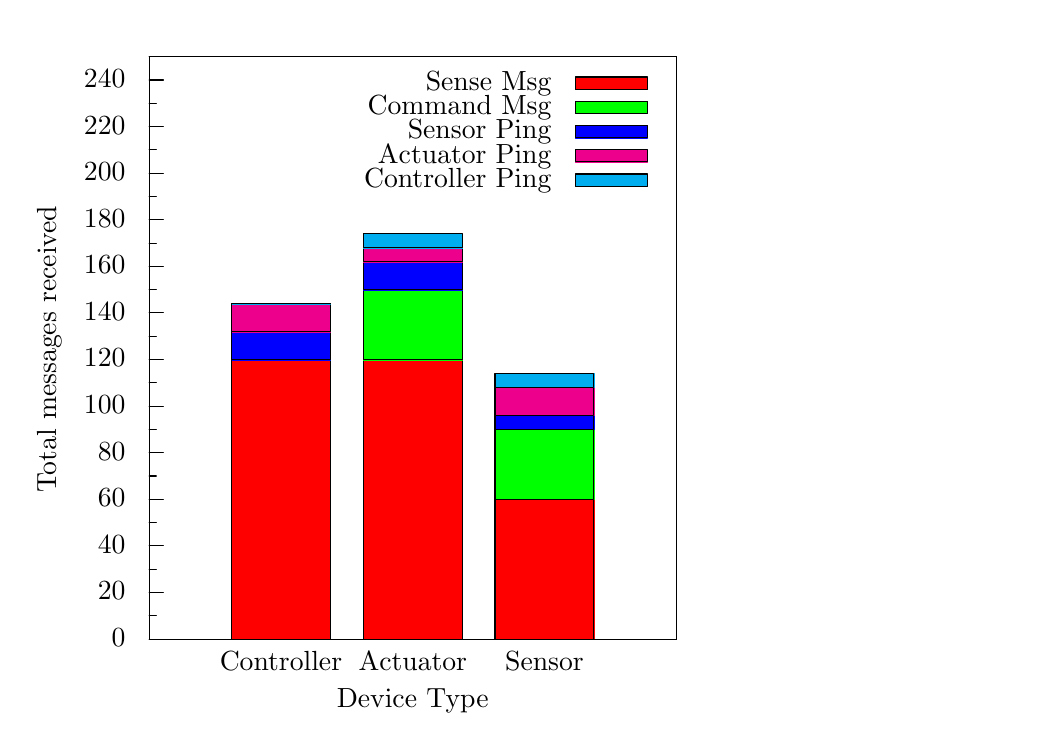
\begin{tikzpicture}[gnuplot]
%% generated with GNUPLOT 4.7p0 (Lua 5.1; terminal rev. 99, script rev. 100)
%% Wed 15 May 2013 18:37:35 BST
\gpsolidlines
\path (0.000,0.000) rectangle (12.500,8.750);
\gpcolor{color=gp lt color border}
\gpsetlinetype{gp lt border}
\gpsetlinewidth{1.00}
\draw[gp path] (1.504,0.985)--(1.684,0.985);
\node[gp node right] at (1.320,0.985) { 0};
\draw[gp path] (1.504,1.281)--(1.594,1.281);
\draw[gp path] (1.504,1.577)--(1.684,1.577);
\node[gp node right] at (1.320,1.577) { 20};
\draw[gp path] (1.504,1.873)--(1.594,1.873);
\draw[gp path] (1.504,2.168)--(1.684,2.168);
\node[gp node right] at (1.320,2.168) { 40};
\draw[gp path] (1.504,2.464)--(1.594,2.464);
\draw[gp path] (1.504,2.760)--(1.684,2.760);
\node[gp node right] at (1.320,2.760) { 60};
\draw[gp path] (1.504,3.056)--(1.594,3.056);
\draw[gp path] (1.504,3.352)--(1.684,3.352);
\node[gp node right] at (1.320,3.352) { 80};
\draw[gp path] (1.504,3.648)--(1.594,3.648);
\draw[gp path] (1.504,3.943)--(1.684,3.943);
\node[gp node right] at (1.320,3.943) { 100};
\draw[gp path] (1.504,4.239)--(1.594,4.239);
\draw[gp path] (1.504,4.535)--(1.684,4.535);
\node[gp node right] at (1.320,4.535) { 120};
\draw[gp path] (1.504,4.831)--(1.594,4.831);
\draw[gp path] (1.504,5.127)--(1.684,5.127);
\node[gp node right] at (1.320,5.127) { 140};
\draw[gp path] (1.504,5.423)--(1.594,5.423);
\draw[gp path] (1.504,5.718)--(1.684,5.718);
\node[gp node right] at (1.320,5.718) { 160};
\draw[gp path] (1.504,6.014)--(1.594,6.014);
\draw[gp path] (1.504,6.310)--(1.684,6.310);
\node[gp node right] at (1.320,6.310) { 180};
\draw[gp path] (1.504,6.606)--(1.594,6.606);
\draw[gp path] (1.504,6.902)--(1.684,6.902);
\node[gp node right] at (1.320,6.902) { 200};
\draw[gp path] (1.504,7.198)--(1.594,7.198);
\draw[gp path] (1.504,7.493)--(1.684,7.493);
\node[gp node right] at (1.320,7.493) { 220};
\draw[gp path] (1.504,7.789)--(1.594,7.789);
\draw[gp path] (1.504,8.085)--(1.684,8.085);
\node[gp node right] at (1.320,8.085) { 240};
\draw[gp path] (1.504,8.381)--(1.594,8.381);
\draw[gp path] (3.177,0.985)--(3.177,1.165);
\node[gp node center] at (3.177,0.677) {Controller};
\draw[gp path] (4.851,0.985)--(4.851,1.165);
\node[gp node center] at (4.851,0.677) {Actuator};
\draw[gp path] (6.524,0.985)--(6.524,1.165);
\node[gp node center] at (6.524,0.677) {Sensor};
\draw[gp path] (1.504,8.381)--(1.504,0.985)--(8.197,0.985)--(8.197,8.381)--cycle;
\node[gp node center,rotate=-270] at (0.246,4.683) {Total messages received};
\node[gp node center] at (4.850,0.215) {Device Type};
\node[gp node right] at (6.729,8.047) {Sense Msg};
\gpfill{color=gp lt color 0} (6.913,7.970)--(7.829,7.970)--(7.829,8.124)--(6.913,8.124)--cycle;
\gpsetlinetype{gp lt plot 0}
\draw[gp path] (6.913,7.970)--(7.829,7.970)--(7.829,8.124)--(6.913,8.124)--cycle;
\gpfill{color=gp lt color 0} (2.550,0.985)--(3.806,0.985)--(3.806,4.536)--(2.550,4.536)--cycle;
\draw[gp path] (2.550,0.985)--(2.550,4.535)--(3.805,4.535)--(3.805,0.985)--cycle;
\gpfill{color=gp lt color 0} (4.223,0.985)--(5.479,0.985)--(5.479,4.536)--(4.223,4.536)--cycle;
\draw[gp path] (4.223,0.985)--(4.223,4.535)--(5.478,4.535)--(5.478,0.985)--cycle;
\gpfill{color=gp lt color 0} (5.896,0.985)--(7.152,0.985)--(7.152,2.761)--(5.896,2.761)--cycle;
\draw[gp path] (5.896,0.985)--(5.896,2.760)--(7.151,2.760)--(7.151,0.985)--cycle;
\node[gp node right] at (6.729,7.739) {Command Msg};
\gpfill{color=gp lt color 1} (6.913,7.662)--(7.829,7.662)--(7.829,7.816)--(6.913,7.816)--cycle;
\gpsetlinetype{gp lt plot 1}
\draw[gp path] (6.913,7.662)--(7.829,7.662)--(7.829,7.816)--(6.913,7.816)--cycle;
\gpfill{color=gp lt color 1} (2.550,4.535)--(3.806,4.535)--(3.806,4.536)--(2.550,4.536)--cycle;
\draw[gp path] (2.550,4.535)--(3.805,4.535)--cycle;
\gpfill{color=gp lt color 1} (4.223,4.535)--(5.479,4.535)--(5.479,5.424)--(4.223,5.424)--cycle;
\draw[gp path] (4.223,4.535)--(4.223,5.423)--(5.478,5.423)--(5.478,4.535)--cycle;
\gpfill{color=gp lt color 1} (5.896,2.760)--(7.152,2.760)--(7.152,3.649)--(5.896,3.649)--cycle;
\draw[gp path] (5.896,2.760)--(5.896,3.648)--(7.151,3.648)--(7.151,2.760)--cycle;
\node[gp node right] at (6.729,7.431) {Sensor Ping};
\gpfill{color=gp lt color 2} (6.913,7.354)--(7.829,7.354)--(7.829,7.508)--(6.913,7.508)--cycle;
\gpsetlinetype{gp lt plot 2}
\draw[gp path] (6.913,7.354)--(7.829,7.354)--(7.829,7.508)--(6.913,7.508)--cycle;
\gpfill{color=gp lt color 2} (2.550,4.535)--(3.806,4.535)--(3.806,4.891)--(2.550,4.891)--cycle;
\draw[gp path] (2.550,4.535)--(2.550,4.890)--(3.805,4.890)--(3.805,4.535)--cycle;
\gpfill{color=gp lt color 2} (4.223,5.423)--(5.479,5.423)--(5.479,5.779)--(4.223,5.779)--cycle;
\draw[gp path] (4.223,5.423)--(4.223,5.778)--(5.478,5.778)--(5.478,5.423)--cycle;
\gpfill{color=gp lt color 2} (5.896,3.648)--(7.152,3.648)--(7.152,3.826)--(5.896,3.826)--cycle;
\draw[gp path] (5.896,3.648)--(5.896,3.825)--(7.151,3.825)--(7.151,3.648)--cycle;
\node[gp node right] at (6.729,7.123) {Actuator Ping};
\gpfill{color=gp lt color 3} (6.913,7.046)--(7.829,7.046)--(7.829,7.200)--(6.913,7.200)--cycle;
\gpsetlinetype{gp lt plot 3}
\draw[gp path] (6.913,7.046)--(7.829,7.046)--(7.829,7.200)--(6.913,7.200)--cycle;
\gpfill{color=gp lt color 3} (2.550,4.890)--(3.806,4.890)--(3.806,5.246)--(2.550,5.246)--cycle;
\draw[gp path] (2.550,4.890)--(2.550,5.245)--(3.805,5.245)--(3.805,4.890)--cycle;
\gpfill{color=gp lt color 3} (4.223,5.778)--(5.479,5.778)--(5.479,5.956)--(4.223,5.956)--cycle;
\draw[gp path] (4.223,5.778)--(4.223,5.955)--(5.478,5.955)--(5.478,5.778)--cycle;
\gpfill{color=gp lt color 3} (5.896,3.825)--(7.152,3.825)--(7.152,4.181)--(5.896,4.181)--cycle;
\draw[gp path] (5.896,3.825)--(5.896,4.180)--(7.151,4.180)--(7.151,3.825)--cycle;
\node[gp node right] at (6.729,6.815) {Controller Ping};
\gpfill{color=gp lt color 4} (6.913,6.738)--(7.829,6.738)--(7.829,6.892)--(6.913,6.892)--cycle;
\gpsetlinetype{gp lt plot 4}
\draw[gp path] (6.913,6.738)--(7.829,6.738)--(7.829,6.892)--(6.913,6.892)--cycle;
\gpfill{color=gp lt color 4} (2.550,5.245)--(3.806,5.245)--(3.806,5.246)--(2.550,5.246)--cycle;
\draw[gp path] (2.550,5.245)--(3.805,5.245)--cycle;
\gpfill{color=gp lt color 4} (4.223,5.955)--(5.479,5.955)--(5.479,6.134)--(4.223,6.134)--cycle;
\draw[gp path] (4.223,5.955)--(4.223,6.133)--(5.478,6.133)--(5.478,5.955)--cycle;
\gpfill{color=gp lt color 4} (5.896,4.180)--(7.152,4.180)--(7.152,4.359)--(5.896,4.359)--cycle;
\draw[gp path] (5.896,4.180)--(5.896,4.358)--(7.151,4.358)--(7.151,4.180)--cycle;
\gpsetlinetype{gp lt border}
\draw[gp path] (1.504,8.381)--(1.504,0.985)--(8.197,0.985)--(8.197,8.381)--cycle;
%% coordinates of the plot area
\gpdefrectangularnode{gp plot 1}{\pgfpoint{1.504cm}{0.985cm}}{\pgfpoint{8.197cm}{8.381cm}}
\end{tikzpicture}
%% gnuplot variables

\caption{xAP}
\label{graph:IoT2}
\end{minipage}
\end{figure}


\end{frame}
% section comparison (end)

\section{Is this it?} % (fold)
\label{sec:is_this_it_}
\begin{frame}\frametitle{Getting there...}
\begin{itemize}
  \item[--] \textbf{Some great scalable ideas but}
\begin{itemize}
  \item Needs to be ported across platforms to really test it
  \item Create applications for it
  \item Other power saving ideas, sleepy motes, less transmissions, more readings
\end{itemize}
\item [--] \textbf{Internet of Things will be divided and slowly merge.}
  
\end{itemize}


\end{frame}
\begin{frame}[t]\frametitle{Questions?}

\begin{figure}
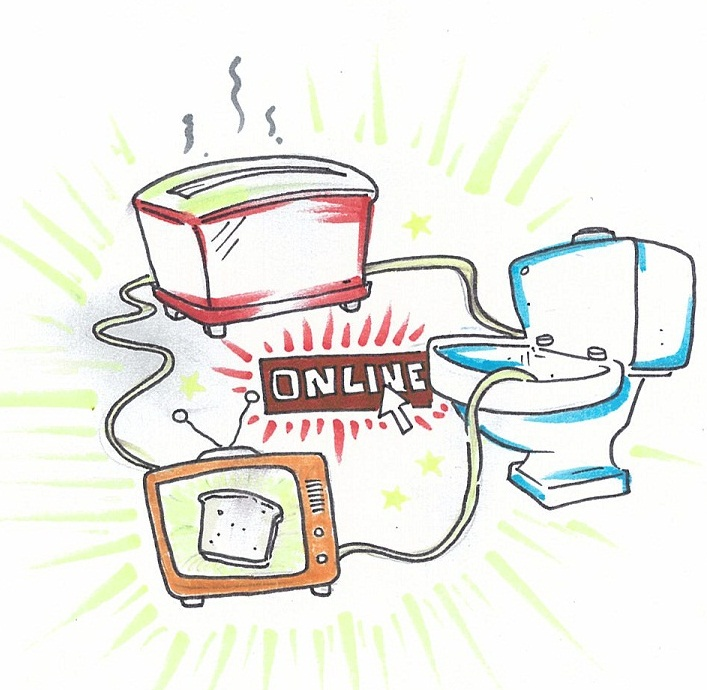
\includegraphics[scale=0.2]{presentation/img/internet-of-things.jpg}
\caption{Connecting everything...\footnote{from http://scribbles-notes.blogspot.co.uk}}

\end{figure}
\end{frame}
% section is_this_it_ (end)
\end{document}